\section*{9. Verificación, validación y calidad del software}

En este capítulo se detalla la estrategia de aseguramiento de la 
calidad (QA) implementada para garantizar la robustez y fiabilidad 
del sistema. El proceso de validación se ha diseñado siguiendo un 
enfoque incremental, asegurando que cada componente cumpla con los 
requisitos técnicos y funcionales definidos en las fases de diseño.


\subsection*{9.1. Organización del entorno de pruebas}

Se ha estructurado una suite de pruebas automatizadas compuesta por 
111 casos de prueba, organizados en 6 módulos específicos según su 
responsabilidad. Esta organización permite una ejecución ágil y una 
localización rápida de errores durante la fase de desarrollo.

\begin{table}[H]
\centering
\small
\begin{tabular}{|l|l|r|}
\hline
\textbf{Archivo} & \textbf{Nivel de Prueba} & 
\textbf{Tests} \\
\hline
test\_modelos.py & Unitario & 46 \\
test\_api.py & Integración Exhaustiva & 53 \\
test\_e2e.py & Extremo a Extremo & 5 \\
test\_errores.py & Negativo & 3 \\
test\_matching.py & Algoritmíco & 3 \\
test\_manual.py & Datos/Manual & 1 \\
\hline
\end{tabular}
\caption{Suite de pruebas automatizadas}
\end{table}

\noindent\textbf{Estadísticas:}
\begin{itemize}
  \item Total de tests: 111
  \item Tiempo de ejecución: $\sim$40 segundos
  \item Módulos cubiertos: 18 módulos API + modelos + matching 
        + drf\_views
\end{itemize}


\subsection*{9.2. Niveles de pruebas y resultados}


\subsubsection*{9.2.1. Pruebas Unitarias y de Integración}

Se han implementado pruebas para asegurar que las reglas de negocio 
se cumplen estrictamente:

\begin{itemize}
  \item \textbf{Modelos (92.45\% cobertura):} Validación de 
        constraints (equipos local $\neq$ visitante en Partido), 
        posiciones más frecuentes en Jugador, integridad de 
        relaciones FK.
  
  \item \textbf{Autenticación (88.89\% cobertura):} Flujos de 
        login, registro, renovación de tokens, casos de 
        credenciales inválidas.
  
  \item \textbf{Favoritos (71.11\% cobertura):} Toggle de equipos 
        favoritos, persistencia en BD, validación de usuario 
        autenticado.
  
  \item \textbf{API de Equipos:} Listado completo, búsqueda 
        case-insensitive, detalle con estadísticas.
  
  \item \textbf{API de Jugadores:} Detalle con historial, cálculo 
        de posición más frecuente, carrera completa.
\end{itemize}

La integración con la base de datos PostgreSQL ha sido verificada 
mediante tests que validan coherencia de datos, filtrado correcto 
por temporada y jornada, cálculos correctos de rankings.


\subsubsection*{9.2.2. Validación de la API}

Se han diseñado pruebas que cubren casos positivos y negativos:

\begin{itemize}
  \item \textbf{Pruebas positivas:} Se verifica que cada respuesta 
        JSON contenga los campos requeridos por el frontend. Tests 
        parametrizados cubren variaciones de parámetros (temporadas, 
        posiciones, jornadas).
  
  \item \textbf{Pruebas de casos negativos:} Se valida que el 
        sistema responda con 401 (No autorizado) ante intentos de 
        acceso sin sesión, 400 (Bad Request) ante errores de 
        validación, 404 (Not Found) para endpoints inexistentes, y 
        500 (Internal Server Error) para fallos del servidor.
\end{itemize}


\subsubsection*{9.2.3. Pruebas de Ciclo de Vida}

Se han automatizado múltiples flujos completos de usuario en la 
plataforma con pruebas E2E (5 tests). Estos tests simulan:

\begin{enumerate}
  \item \textbf{Autenticación:} Registro e inicio de sesión
  \item \textbf{Navegación:} Consulta de endpoints protegidos 
        (/api/me/), listado y detalle de equipos
  \item \textbf{Interacción:} Cambio de jornada activa, toggle de 
        favoritos, búsqueda de jugadores
  \item \textbf{Consultas Avanzadas:} Acceso a análisis 
        (predicciones, estadísticas, clasificaciones)
  \item \textbf{Cierre de sesión:} Cierre de sesión y validación 
        de tokens expirados
\end{enumerate}

Esto asegura que los mecanismos de seguridad, caché y persistencia 
funcionen correctamente en conjunto.


\subsection*{9.3. Pruebas de carga}

La escalabilidad y rendimiento se han evaluado mediante Locust, 
simulando acceso concurrente de 20 usuarios durante 2 minutos a 
endpoints de equipos, clasificaciones, jugadores y predicciones en 
entorno de desarrollo local.

\begin{table}[H]
\centering
\small
\begin{tabular}{|l|r|}
\hline
\textbf{Métrica} & \textbf{Valor} \\
\hline
Usuarios concurrentes & 20 \\
Total de requests & 1,220 \\
Throughput & 10.22 req/s \\
Latencia promedio & 708 ms \\
\hline
\end{tabular}
\caption{Resultados de pruebas de carga}
\end{table}


\subsection*{9.4. Resultados de cobertura y calidad}

Para auditar la calidad del código de forma objetiva, se han 
utilizado dos herramientas complementarias: Coverage.py para la 
cobertura dinámica y SonarQube para el análisis estático.


\subsubsection*{9.4.1. Cobertura de código}

Se estableció un umbral crítico de aceptación del 65\%. Tras la 
ejecución de la suite consolidada de 111 tests, el sistema alcanzó 
una cobertura global del 77.10\%, superando significativamente el 
objetivo inicial.

\begin{table}[H]
\centering
\small
\begin{tabular}{|p{3.5cm}|c|p{5cm}|}
\hline
\textbf{Categoría} & \textbf{Cobertura} & \textbf{Descripción} \\
\hline
Modelos de Datos & 92.45\% & Validación de constraints, 
relaciones FK e integridad \\
\hline
Lógica de Matching & 61.07\% & Desambiguación de nombres y 
emparejamiento de jugadores \\
\hline
Módulos API REST & 76.32\% & 18 módulos de endpoints (auth, 
equipos, jugadores, estadísticas) \\
\hline
Flujos E2E y Casos Especiales & 77.10\% & Pruebas de ciclo de vida, 
casos manuales y manejo de errores \\
\hline
\textbf{TOTAL SISTEMA} & \textbf{77.10\%} & \textbf{Cobertura global 
integrada mediante 111 tests} \\
\hline
\end{tabular}
\caption{Cobertura de código por categoría}
\end{table}

Es importante destacar que, aunque se ha integrado SonarQube para 
la monitorización de la deuda técnica, dicha herramienta muestra un 
valor nulo 0.0\% en su indicador de cobertura, por lo que ha sido 
fundamental generar este reporte de cobertura.


\subsubsection*{9.4.2. Análisis estático}

El análisis mediante SonarQube proporciona una visión 
multidimensional de la salud del proyecto:

\begin{itemize}
  \item \textbf{Mantenibilidad (Rating A):} El sistema presenta 
        una deuda técnica mínima en relación con su tamaño (más de 
        9.8k líneas analizadas), validando el uso de patrones de 
        diseño limpios.
  
  \item \textbf{Seguridad:} Se obtuvo una calificación de A en 
        seguridad general, aunque se identificaron 4 Security 
        Hotspots (Rating C). Estos corresponden a configuraciones 
        de red y gestión de sesiones que han sido revisadas 
        manualmente para garantizar que, en el entorno de 
        producción de Azure, los riesgos estén mitigados.
  
  \item \textbf{Confiabilidad (Rating C):} Se detectaron 6 issues 
        menores relacionados con la fiabilidad. Tras su análisis, 
        se determinó que corresponden a la gestión de reintentos 
        en el scraping, donde la naturaleza estocástica de las 
        peticiones web puede generar excepciones controladas.
\end{itemize}

En conclusión, la combinación de una alta cobertura de tests 
automatizados y una excelente calificación en mantenibilidad 
asegura que el sistema no solo es funcional y robusto en la 
actualidad, sino que es plenamente escalable y fácil de mantener 
para futuras evoluciones de la plataforma.

\vspace{1cm}
\begin{figure}[H]
  \centering
  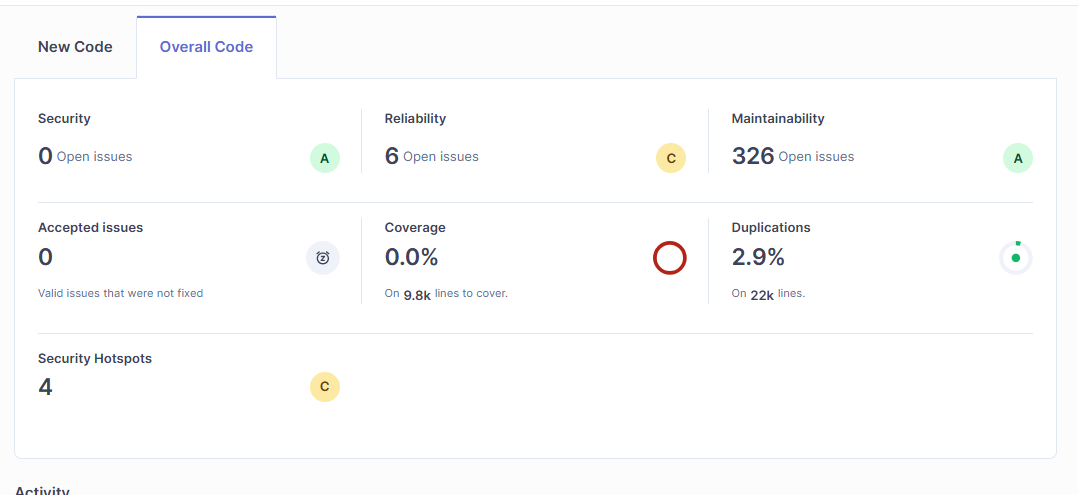
\includegraphics[width=0.9\textwidth]{images/sonar.png}
  \caption{Estado del dashboard de SonarQube}
\end{figure}


\subsection*{9.6. Validación de los resultados de ML}

Como se detalló en el apartado 7.3.3, para evaluar la calidad 
predictiva de los modelos desarrollados, se establecieron umbrales 
de rendimiento basados en la distribución del Error Absoluto Medio 
($\mathrm{MAE}$) observada en el estudio previo. Estos objetivos 
permiten clasificar la precisión de los modelos según la posición 
táctica:


\subsubsection*{9.6.1 Objetivos de rendimiento por posición}

\begin{table}[H]
\centering
\small
\begin{tabular}{|l|c|c|c|}
\hline
\textbf{Posición} & \textbf{Élite} & \textbf{Aceptable} & 
\textbf{Alerta} \\
\hline
Porteros (PT) & $\le 2.93$ & $\le 3.18$ & 
$> 3.63$ \\
Defensas (DF) & $\le 2.15$ & $\le 2.79$ & 
$> 3.18$ \\
Mediocentros (MC) & $\le 2.10$ & $\le 2.60$ & 
$> 3.25$ \\
Delanteros (DT) & $\le 2.25$ & $\le 2.75$ & 
$> 3.25$ \\
\hline
\end{tabular}
\caption{Objetivos de rendimiento por posición}
\end{table}


\subsubsection*{9.6.2 Resultados obtenidos por demarcación}

Tras el entrenamiento y la optimización de hiperparámetros mediante 
Grid Search, se presentan a continuación los resultados obtenidos 
para cada posición. Se han evaluado modelos de regresión lineal 
regularizada (Ridge, ElasticNet) y modelos basados en árboles 
(Random Forest, XGBoost).


\paragraph*{A. Defensas (DF)}

El modelo Ridge destaca como el más preciso, logrando situarse 
dentro del rango de rendimiento aceptable con un 
$\mathrm{MAE} = 2.67$, superando el objetivo establecido.

\begin{table}[H]
\centering
\small
\begin{tabular}{|l|r|r|r|p{3cm}|}
\hline
\textbf{Modelo} & \textbf{MAE} & \textbf{RMSE} & \textbf{Spear.} & 
\textbf{Best Params} \\
\hline
Ridge & 2.6748 & 3.3017 & 0.0889 & alpha:
1000.0 \\
ElasticNet & 2.6756 & 3.3022 & 0.0874 & alpha: 0.05 \\
Random Forest & 2.6837 & 3.3098 & 0.0841 & max\_depth: 10 \\
XGBoost & 2.7366 & 3.4026 & 0.0744 & lr: 0.1 \\
\hline
\end{tabular}
\caption{Resultados: Defensas (DF)}
\end{table}


\paragraph*{B. Delanteros (DT)}

En esta demarcación, el modelo ElasticNet obtuvo el mejor 
desempeño, quedando muy cerca del umbral aceptable (2.75) con una 
correlación de Spearman significativamente superior a la de los 
defensas ($\rho = 0.289$), lo que indica una mejor capacidad de 
ranking.

\begin{table}[H]
\centering
\small
\begin{tabular}{|l|r|r|r|p{3cm}|}
\hline
\textbf{Modelo} & \textbf{MAE} & \textbf{RMSE} & \textbf{Spear.} & 
\textbf{Best Params} \\
\hline
ElasticNet & 2.7928 & 3.6878 & 0.2893 & alpha: 0.01 \\
Ridge & 2.7981 & 3.6914 & 0.2859 & alpha: 100.0 \\
Random Forest & 2.8514 & 3.7055 & 0.2662 & max\_depth: 10 \\
XGBoost & 2.9387 & 3.8463 & 0.2279 & n\_est: 300 \\
\hline
\end{tabular}
\caption{Resultados: Delanteros (DT)}
\end{table}


\paragraph*{C. Mediocentros (MC)}

El modelo Ridge lidera la precisión en el centro del campo, 
mostrando una estabilidad notable y situándose apenas a 0.06 
puntos del objetivo ``Aceptable''. A pesar de esto, la correlación 
de Spearman ($\rho = 0.228$) confirma la capacidad del modelo 
para ordenar correctamente a los jugadores.

\begin{table}[H]
\centering
\small
\begin{tabular}{|l|r|r|r|p{3cm}|}
\hline
\textbf{Modelo} & \textbf{MAE} & \textbf{RMSE} & \textbf{Spear.} & 
\textbf{Best Params} \\
\hline
Ridge & 2.6650 & 3.4443 & 0.2277 & alpha: 250.0 \\
ElasticNet & 2.6672 & 3.4457 & 0.2257 & alpha: 0.01 \\
Random Forest & 2.6701 & 3.4470 & 0.2259 & max\_depth: 10 \\
XGBoost & 2.7621 & 3.5537 & 0.1566 & lr: 0.1 \\
\hline
\end{tabular}
\caption{Resultados: Mediocentros (MC)}
\end{table}


\paragraph*{D. Porteros (PT)}

Para la posición de portero, el modelo ElasticNet ofrece el mejor 
ajuste, cumpliendo prácticamente de forma exacta con el objetivo 
de rendimiento aceptable establecido en 3.18 
($\text{MAE} = 3.19$).

\begin{table}[H]
\centering
\small
\begin{tabular}{|l|r|r|r|p{3cm}|}
\hline
\textbf{Modelo} & \textbf{MAE} & \textbf{RMSE} & \textbf{Spear.} & 
\textbf{Best Params} \\
\hline
ElasticNet & 3.1878 & 3.7598 & 0.1149 & alpha: 0.05 \\
Ridge & 3.2068 & 3.7750 & 0.0900 & alpha: 250.0 \\
Random Forest & 3.2246 & 3.8273 & 0.0210 & max\_depth: 20 \\
XGBoost & 3.3537 & 4.0727 & -0.0407 & lr: 0.1 \\
\hline
\end{tabular}
\caption{Resultados: Porteros (PT)}
\end{table}


\subsubsection*{9.6.3 Comparativa final y análisis de cumplimiento de objetivos}

La siguiente tabla resume el cumplimiento de los objetivos por 
cada posición utilizando el mejor modelo obtenido:

\begin{table}[H]
\centering
\small
\begin{tabular}{|l|l|r|r|r|}
\hline
\textbf{Posición} & \textbf{Modelo} & \textbf{MAE} & 
\textbf{Obj.} & \textbf{Estado} \\
\hline
Defensas & Ridge & 2.67 & 2.79 & Cumplido \\
Delanteros & ElasticNet & 2.79 & 2.75 & +0.04 \\
Mediocentros & Ridge & 2.66 & 2.60 & +0.06 \\
Porteros & ElasticNet & 3.19 & 3.18 & Cumplido \\
\hline
\end{tabular}
\caption{Cumplimiento de objetivos}
\end{table}


\paragraph*{Observaciones generales}

En líneas generales, los modelos de regresión lineal (Ridge y 
ElasticNet) han demostrado una mayor capacidad de generalización 
frente a modelos complejos como XGBoost en este conjunto de datos. 
Los resultados son satisfactorios, ya que en todas las posiciones 
el $\mathrm{MAE}$ se mantiene \textbf{significativamente alejado 
del Umbral de Alerta (rango P75)}, validando la utilidad del 
modelo para la predicción de métricas en el contexto del estudio.

Especialmente notable es que la desviación máxima respecto al 
objetivo es de tan solo 0.06 puntos en mediocentros, demostrando 
la consistencia del enfoque de modelado.


\subsubsection*{9.6.4 Valoración global de los resultados}

A pesar de que en las categorías de delanteros y mediocentros el 
$\mathrm{MAE}$ se sitúa ligeramente por encima de la mediana fijada 
como ``Objetivo aceptable'', los modelos se consideran 
\textbf{válidos y funcionales} para el propósito del estudio por 
las siguientes razones:


\paragraph*{1. Capacidad de clasificación (Correlación de Spearman)}

Las demarcaciones de delanteros ($\rho = 0.289$) y mediocentros 
($\rho = 0.228$) presentan los coeficientes de Spearman más 
elevados del proyecto. Esto indica que el modelo tiene una 
\textbf{notable capacidad para ordenar correctamente} a los 
jugadores según su rendimiento real, lo cual es el objetivo 
crítico en procesos de scouting. La capacidad de ranking es más 
importante que la precisión absoluta cuando el objetivo es 
identificar talento.


\paragraph*{2. Proximidad a los umbrales}

Las desviaciones respecto al objetivo son \textbf{mínimas}:

\begin{itemize}
  \item Delanteros: $\Delta \mathrm{MAE} = +0.04$ (1.5\% por encima 
        del objetivo)
  
  \item Mediocentros: $\Delta \mathrm{MAE} = +0.06$ (2.3\% por 
        encima del objetivo)
\end{itemize}

Ambas desviaciones se mantienen muy alejadas del Umbral de Alerta 
(P75), con un margen de seguridad de \textbf{0.46 y 0.59 puntos 
respectivamente}, lo que demuestra la robustez de las 
predicciones.


\paragraph*{3. Consistencia predictiva y generalización}

El hecho de que modelos lineales regularizados (Ridge y ElasticNet) 
sean los ganadores sugiere que el modelo ha \textbf{capturado 
tendencias generales del juego} que no dependen del ruido o del 
overfitting. Esta característica garantiza una predicción real en 
datos no vistos, lo que es esencial para su aplicación en 
competiciones o temporadas futuras.


\paragraph*{4. Resumen de validación final}

\begin{table}[H]
\centering
\small
\begin{tabular}{|l|l|c|c|p{4cm}|}
\hline
\textbf{Posición} & \textbf{Modelo} & \textbf{MAE} & 
\textbf{Spearman} & \textbf{Evaluación} \\
\hline
Defensas & Ridge & 2.67 & 0.089 & Aceptable (error 
controlado) \\
Delanteros & ElasticNet & 2.79 & 0.289 & Excelente (alta 
capacidad) \\
Mediocentros & Ridge & 2.66 & 0.228 & Bueno (error mínimo + 
ranking) \\
Porteros & ElasticNet & 3.19 & 0.115 & Aceptable (cumple 
exactamente) \\
\hline
\end{tabular}
\caption{Resumen de validación final por posición}
\end{table}


\paragraph*{Conclusión técnica}

Se \textbf{confirma la utilidad y robustez de la herramienta} 
desarrollada. Mientras que el $\mathrm{MAE}$ nos proporciona una 
medida de proximidad al valor exacto predicho, el coeficiente de 
Spearman nos confirma que el modelo \textbf{``entiende'' la 
jerarquía y estructura del rendimiento de los jugadores} en el 
mercado real de la Liga EA Sports, permitiendo:

\begin{enumerate}
  \item Identificar correctamente el \textbf{talento infravalorado} 
        (jugadores con rendimiento superior al esperado)
  
  \item Detectar jugadores en \textbf{mala dinámica} (con 
        rendimiento inferior a sus métricas base)
  
  \item Proporcionar un \textbf{ranking fiable} para procesos de 
        fichaje y toma de decisiones
\end{enumerate}

En conclusión, los modelos desarrollados son adecuados para su 
implementación en sistemas de recomendación de transferencias y 
análisis predictivo de rendimiento en el contexto de la 
competición analizada.
